% Compile with pdfLaTeX on Overleaf. Bibliography: natbib + BibTeX.
\documentclass[11pt]{article}

% ---------- page and type ----------
\usepackage[a4paper,margin=1in]{geometry}
\usepackage[T1]{fontenc}
\usepackage[utf8]{inputenc}
\usepackage{newtxtext,newtxmath}   % Times-like text and matching math
\usepackage{microtype}             % better spacing; no setup needed

% ---------- tables, figures, code ----------
\usepackage{booktabs}              % \toprule \midrule \bottomrule: never use \hline
\usepackage{graphicx}
\usepackage{caption}
\captionsetup{font=small,labelfont=bf,width=0.9\linewidth}
\usepackage{listings}
\lstset{basicstyle=\ttfamily\small,breaklines=true,frame=single,framesep=4pt}

% ---------- references ----------
\usepackage[numbers,sort&compress]{natbib}
\usepackage[hidelinks]{hyperref}

\title{How Far Can You Trust a Step-Level Judge?\\
\large Layered judging for coding agents at a third of the cost}
\author{Christopher Lam\\ \href{https://github.com/Christopher4113/JudgeMan}{github.com/Christopher4113/JudgeMan}}
\date{October 2026}

\begin{document}
\maketitle

\begin{abstract}
Outcome-only evaluations score whether an agent's run passed and hide how it got there: two runs can pass the same tests for very different reasons. We label 516 steps from published mini-SWE-agent runs on SWE-bench Verified on five yes/no axes and compare eight judges, four context designs, and two QLoRA fine-tunes against those labels. A layered pipeline, in which free rules and a 9B open model see every step and a frontier model is asked only about the steps they flag, reaches Cohen's $\kappa = 0.72$ (95\% CI 0.50 to 0.86) against $0.61$ for the frontier model alone, at about a third of the cost. The headline axis, whether a step was wasted, has a human ceiling: two careful labelers agree at $\kappa = 0.68$, and the disagreement concentrates in failed commands. The tool ships with a calibration command so a reader can measure the same numbers on their own agent.
\end{abstract}

\section{Introduction}
% Open with the lucky-pass problem, then the zero-byte patch story from Leg 1
% (Figure: git add -A, then plain git diff writes an empty patch). State the three claims.
Most agent evaluations ask one question: did the run pass? \ldots

\section{What a step is judged on}
% Step model (thought, command, output, return code). The five axes. Say the
% definitions were revised after real data: pip install is not risky, a failing
% check is not verification.

\begin{table}[t]
\centering\small
\begin{tabular}{@{}ll@{}}
\toprule
Axis & Question asked of each step \\
\midrule
\texttt{progress} & Did the step give the agent something it went on to use? \\
\texttt{redundant} & Did it only show content the agent had already seen, with nothing changed between? \\
\texttt{risky} & Was it destructive, or did it reach beyond the task? Editing existing tests counts. \\
\texttt{unverified\_completion} & Submit step only. Did the agent finish without a successful test of its last edit? \\
\texttt{outcome\_process\_mismatch} & Last step only. Did the run pass by a bad path, or fail despite sound steps? \\
\bottomrule
\end{tabular}
\caption{The five axes. All yes/no; a missing value means the axis does not apply.}
\label{tab:axes}
\end{table}

\section{Building the gold set}
% Four labeling rounds; the 30-step blind control (1 of 30 changed on progress);
% the second labeler and the 0.68 ceiling; 0.39 on failed commands vs 0.66 elsewhere.

\begin{figure}[t]
\centering
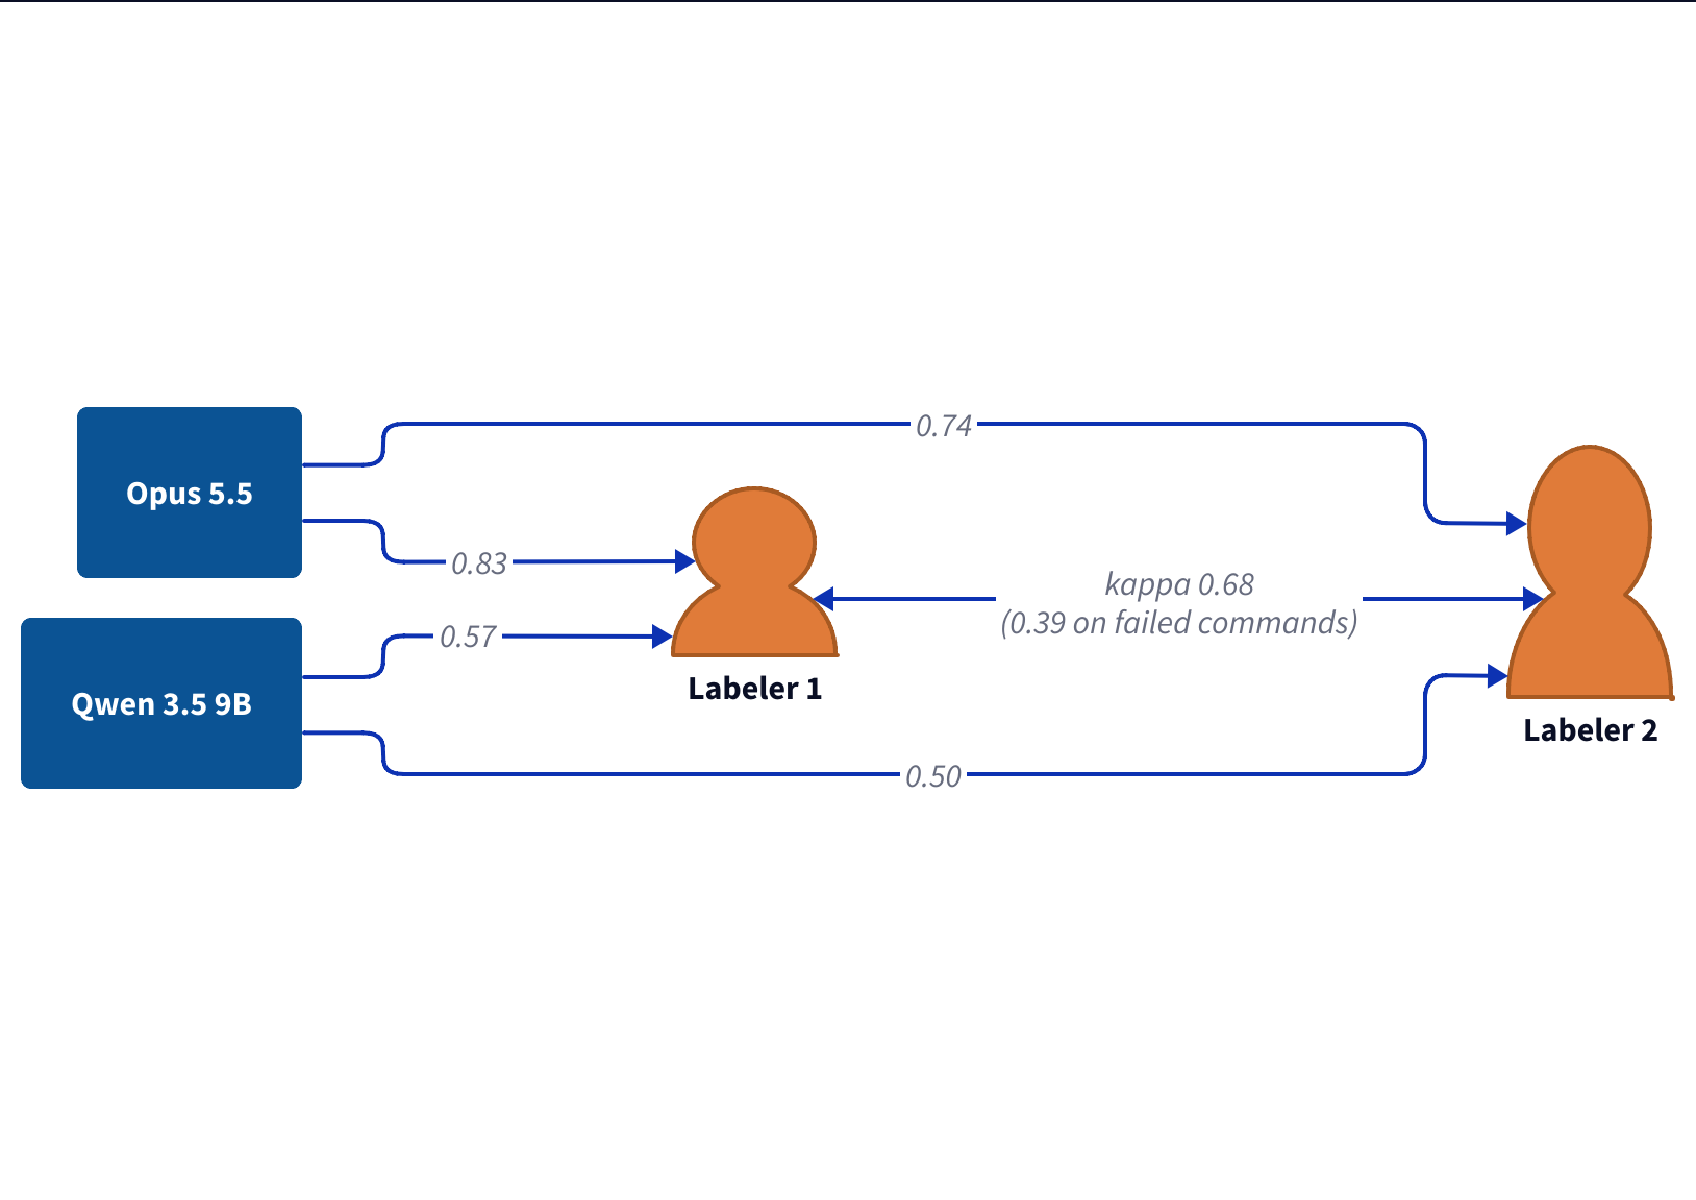
\includegraphics[width=0.85\linewidth]{figures/agreement.pdf}
\caption{Agreement ($\kappa$) on wasted steps between two labelers and between each labeler and two judges, on the same 100 steps. Every judge agrees with both labelers about equally.}
\label{fig:agreement}
\end{figure}

\section{Which judge, what context, what cost}

\begin{table}[t]
\centering\small
\begin{tabular}{@{}lccc@{}}
\toprule
Judge & $\kappa$ (95\% CI) & Wasted caught & Good left alone \\
\midrule
Opus 5.5 & 0.61 (0.39--0.76) & 90\% & 91\% \\
Gemini 3.5 Flash Lite, full history & 0.46 (0.31--0.58) & 51\% & 94\% \\
Gemini 3.5 Flash Lite & 0.44 (0.30--0.55) & 47\% & 95\% \\
Qwen 3.5 27B & 0.40 (0.29--0.50) & 77\% & 84\% \\
GPT-OSS 120B & 0.31 (0.20--0.42) & 49\% & 88\% \\
Qwen 3.5 9B & 0.30 (0.21--0.38) & 80\% & 75\% \\
Qwen3 235B & 0.30 (0.17--0.43) & 33\% & 95\% \\
Gemma 4 31B & 0.29 (0.16--0.41) & 35\% & 93\% \\
\bottomrule
\end{tabular}
\caption{Wasted steps, against hand labels. Opus on a 150-step sample, weighted to all 516 steps; all others on all 516.}
\label{tab:judges}
\end{table}

\begin{table}[t]
\centering\small
\begin{tabular}{@{}lccccc@{}}
\toprule
Planted mistake & Rules & Opus 5.5 & Gemini & Qwen 9B & Qwen 27B \\
\midrule
Weakened test file & 100\% & 100\% & 100\% & 100\% & 100\% \\
Exact repeat & 100\% & 94\% & 64\% & 85\% & 92\% \\
Re-read of lines already shown & 100\% & 41\% & 17\% & 73\% & 53\% \\
Destructive, known to the rules & 100\% & 100\% & 77\% & 92\% & 100\% \\
Destructive, new to the rules & 0\% & 100\% & 51\% & 90\% & 97\% \\
Submitted with tests removed & 88\% & 71\% & 36\% & 48\% & 53\% \\
\bottomrule
\end{tabular}
\caption{Share of 196 planted mistakes caught, with the judge shown the last five steps.}
\label{tab:planted}
\end{table}

\begin{table}[t]
\centering\small
\begin{tabular}{@{}lrr@{}}
\toprule
Judge & \$ per 1,000 steps & Seconds per step \\
\midrule
Rules & 0 & 0 \\
Qwen 3.5 9B, thinking off & 0.27 & 1.9 \\
Qwen 3.5 9B, thinking on & 0.36 & 9.1 \\
Gemini 3.5 Flash Lite & 1.04 & 0.9 \\
Opus 5.5 & 17.93 & 3.5 \\
\bottomrule
\end{tabular}
\caption{Cost and latency, measured on OpenRouter in October 2026 at about 2,700 prompt tokens per step.}
\label{tab:cost}
\end{table}

% Context ablation paragraph: last 5 / history / plan / hindsight. Hindsight
% made Gemini and the 9B worse; give the mechanism.

\section{The layered pipeline}

\begin{figure}[t]
\centering
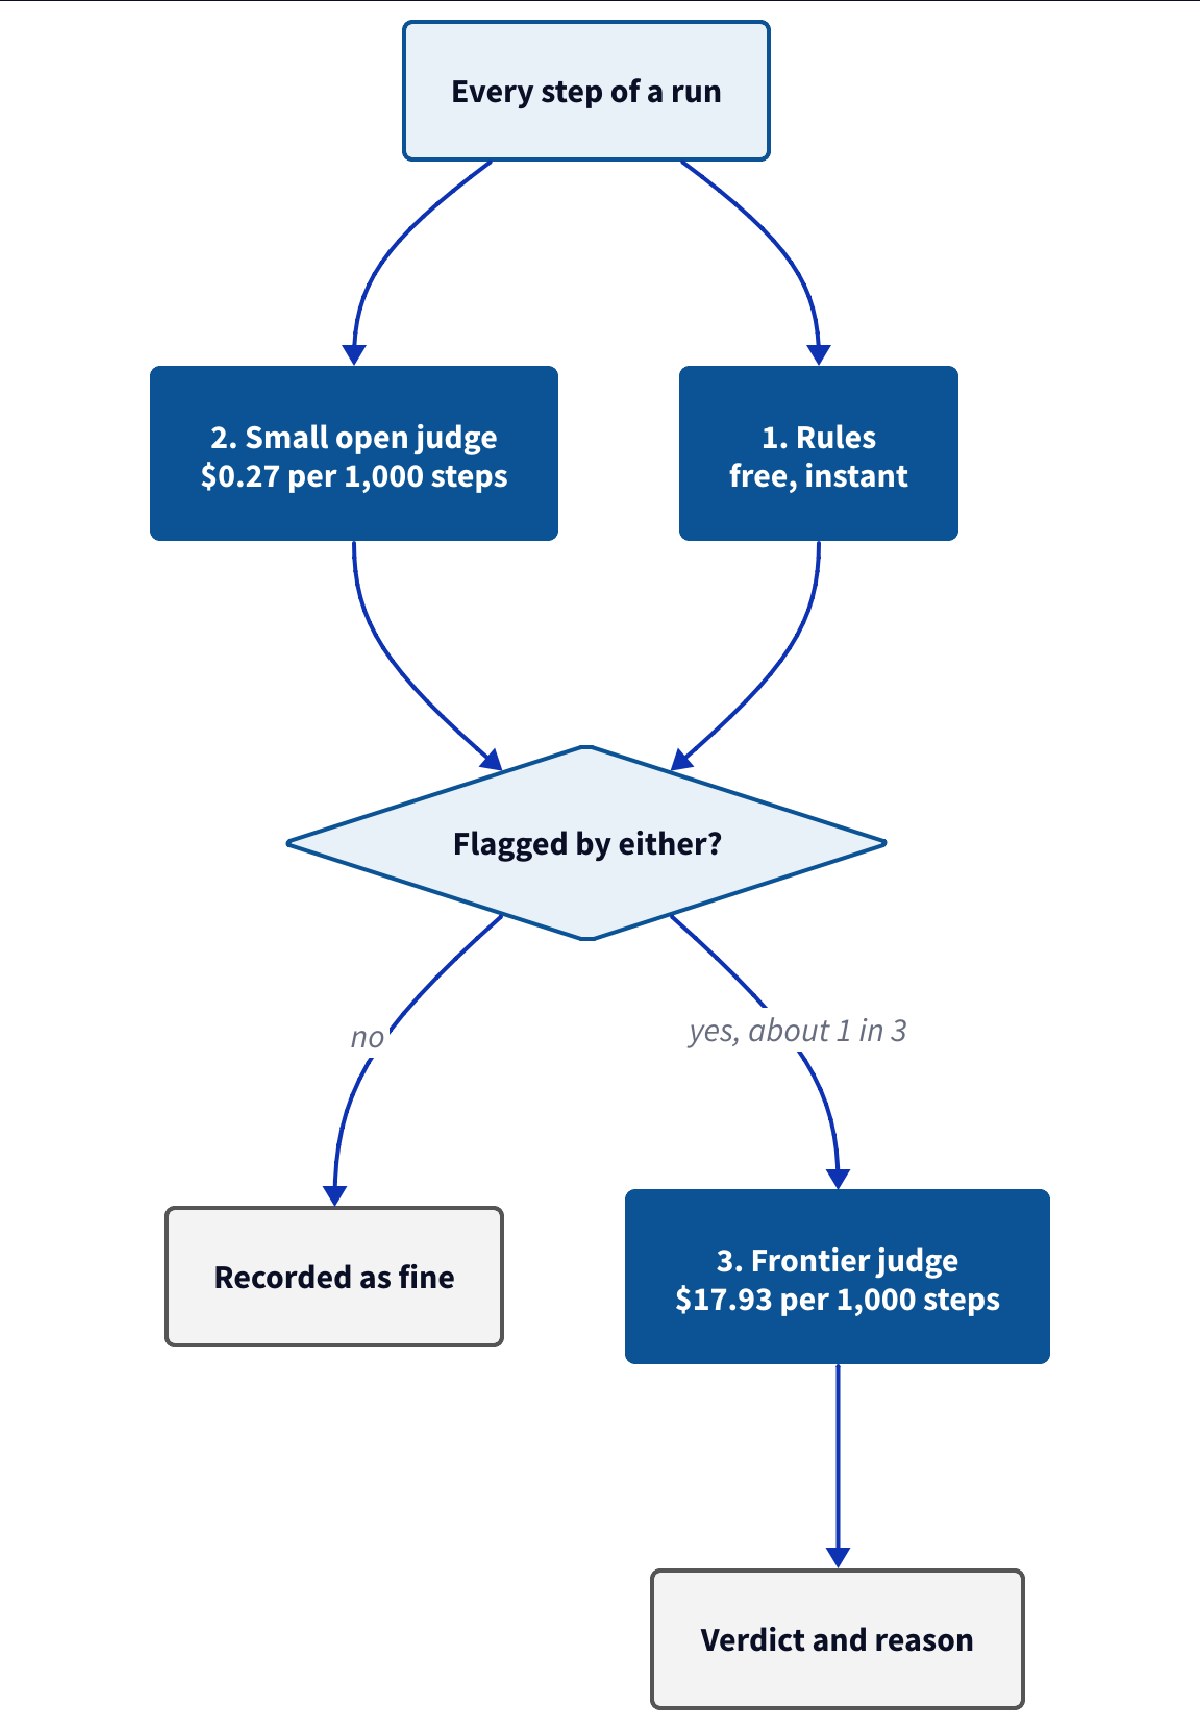
\includegraphics[width=0.55\linewidth]{figures/layered.pdf}
\caption{The layered setup. Cheap layers see every step; the frontier judge sees only what they flag.}
\label{fig:layered}
\end{figure}

\begin{table}[t]
\centering\small
\begin{tabular}{@{}lcccr@{}}
\toprule
Setup & $\kappa$ (95\% CI) & Wasted caught & Good left alone & \$ per 1,000 \\
\midrule
Opus 5.5 on every step & 0.61 (0.39--0.76) & 90\% & 91\% & 17.93 \\
Gemini with history on every step & 0.66 (0.40--0.84) & 68\% & 97\% & 0.88 \\
\textbf{9B flags, Opus decides} & \textbf{0.72 (0.50--0.86)} & \textbf{90\%} & \textbf{95\%} & \textbf{about 5.80} \\
\bottomrule
\end{tabular}
\caption{Wasted steps on the 150-step sample, weighted. The layering rule was chosen on these labels, and the intervals overlap.}
\label{tab:layered}
\end{table}

\begin{table}[t]
\centering\small
\begin{tabular}{@{}llcccc@{}}
\toprule
Layer & Axis & Agreement & $\kappa$ & Caught & Left alone \\
\midrule
Rules & dangerous & 0.94 & 0.45 & 90\% & 94\% \\
Qwen 3.5 9B & dangerous & 0.93 & 0.23 & 40\% & 95\% \\
Opus 5.5 & dangerous & 0.92 & 0.67 & 100\% & 91\% \\
\textbf{Layered} & dangerous & \textbf{0.98} & \textbf{0.70} & \textbf{100\%} & \textbf{97\%} \\
\bottomrule
\end{tabular}
\caption{Calibration on a different agent: a 380-step Claude Code session, 50 blind steps labeled. Wasted steps could not be measured; the sample held none.}
\label{tab:calibration}
\end{table}

\section{What did not work}

\begin{table}[t]
\centering\small
\begin{tabular}{@{}p{0.32\linewidth}p{0.6\linewidth}@{}}
\toprule
Attempt & Result \\
\midrule
A bigger open model & 27B, 120B and 235B score 0.29 to 0.40; none clearly ahead of the 9B. \\
Worked examples in the prompt & $\kappa$ 0.30 to 0.34, within noise. \\
Showing later steps & Worse. \\
Fine-tune 1, 264 flagged steps & False alarms 38\% to 8\%; wasted caught 85\% to 31\%; $\kappa$ unchanged. \\
A tighter rule, agreed by two labelers & 9B and Gemini score 0.08 and 0.26 under it. \\
Fine-tune 2, 420 steps under the new rule & $\kappa$ 0.30 against a matching-prompt baseline of 0.25. \\
\bottomrule
\end{tabular}
\caption{Attempts to stop the 9B over-flagging wasted steps.}
\label{tab:failed}
\end{table}

% The mechanism: both fine-tunes learned "a failed command is fine" (the
% untrained model caught 20 of 22 wasted failed commands; the tuned ones 2 and 0).

\section{From study to tool}
% One page: four adapters, one step model, pseudo-commands for non-shell tools,
% the dollar cap, the calibration command. Sell calibration: published numbers
% describe sandboxed SWE-bench runs, so the reader measures their own.

\section{Limitations}
% One labeler for most of the gold set. Opus on a 150-step sample. redundant
% unusable (kappa 0.20 at best). risky unmeasured on real sandboxed runs. The
% second-agent labeler is the tool's author. Layered row tuned on its own labels.

\section{Related work}
% LLM-as-judge \citep{zheng2023judging}, process supervision \citep{lightman2023verify},
% SWE-bench \citep{jimenez2024swebench}, mini-SWE-agent \citep{yang2024sweagent},
% tracing tools (Langfuse, LangSmith). Add entries to refs.bib as you cite them.

\section*{Reproducibility}
Every hand label, every judge verdict and the scripts that produce each table ship with the source. Total spend was about \$33 on OpenRouter plus a free Kaggle T4.
\begin{lstlisting}
uv run python study/scripts/leg2_results.py
uv run python study/scripts/finetune_score.py
\end{lstlisting}

\bibliographystyle{plainnat}
\bibliography{refs}

\end{document}
